Modificando ulteriormente l'\textit{inseguitore di forza} si pu\'{o} implementare un'applicazione 
per il trasposto collaborativo uomo-robot\footnotemark{}. 
In tale applicazione uomo e robot collaborano per muovere una lamina in fibra di carbonio da una posizione iniziale fino ad uno stampo 
di lavorazione: l'operatore tiene un lembo del materiale mentre il robot tiene l'altra estremit\'{a} attraverso una ventosa. 
L'operatore, tirando a s\'{e} la lamina, fa s\'{i} che il robot segua le sue intenzioni di movimento agevolando lo spostamento del materiale.
Rispetto alla versione utilizzata nella Sezione \ref{sec:force_follower} \'{e} stata aggiunta 
la lettura delle torsioni misurate dal sensore. 
Ad esempio, nel pick and place, le torsioni lungo l'asse z venivano interpretate come l'input da parte dell'operatore per il salvataggio 
delle posizioni. In questo caso, invece, quando il sensore misura una torsione, essa viene interpretata come la volont\'{a} 
dell'operatore di ruotare il pezzo che viene trasportato.
Allo stesso modo delle forze, viene calcolata la \textbf{velocit\'{a} angolare} 
con cui far ruotare l'end effector dell'UR5, in modo tale da riuscire a seguire tutte le intenzioni dell'utente. 
La possibilit\'{a} di rotazione dell'end effector porta, per\'{o}, ad un problema con i sistemi di riferimento. 
Infatti, \verb|twist_controller|, effettua i movimenti rispetto al sistema di riferimento dell'end effector, ma se esso viene ruotato 
sar\'{a} necessario cambiare il verso di movimento per seguire correttamente le forze in input. Per ovviare a questo 
problema, sono state utilizzate le \textbf{trasformazioni geometriche} da un sistema di riferimento ad un altro \cite{foote2013tf}. 
Utilizzando la libreria \verb|tf| di ROS, \'{e} possibile convertire le coordinate di un punto in un sistema di riferimento, nelle 
coordinate di un altro sistema di riferimento connesso ad esso. In questo modo \'{e} stato possibile inviare i comandi 
\verb|Twist| al robot, rispetto ad un sistema di riferimento fisso (quale la base del robot), in modo tale che il vettore velocit\'{a} 
calcolato non fosse dipendente dall'orientazione dell'end effector. 
In questa applicazione si \'{e} sostituito il gripper con delle ventose collegate ad un compressore che, attraverso la creazione di 
una forza di aspirazione, permette al robot di sollevare oggetti sottili e fragili come una lamina di carbonio (vedi Figura \ref{fig:co-op}).
\begin{figure}[H]
    \centering
    \begin{subfigure}[b]{0.45\textwidth}
        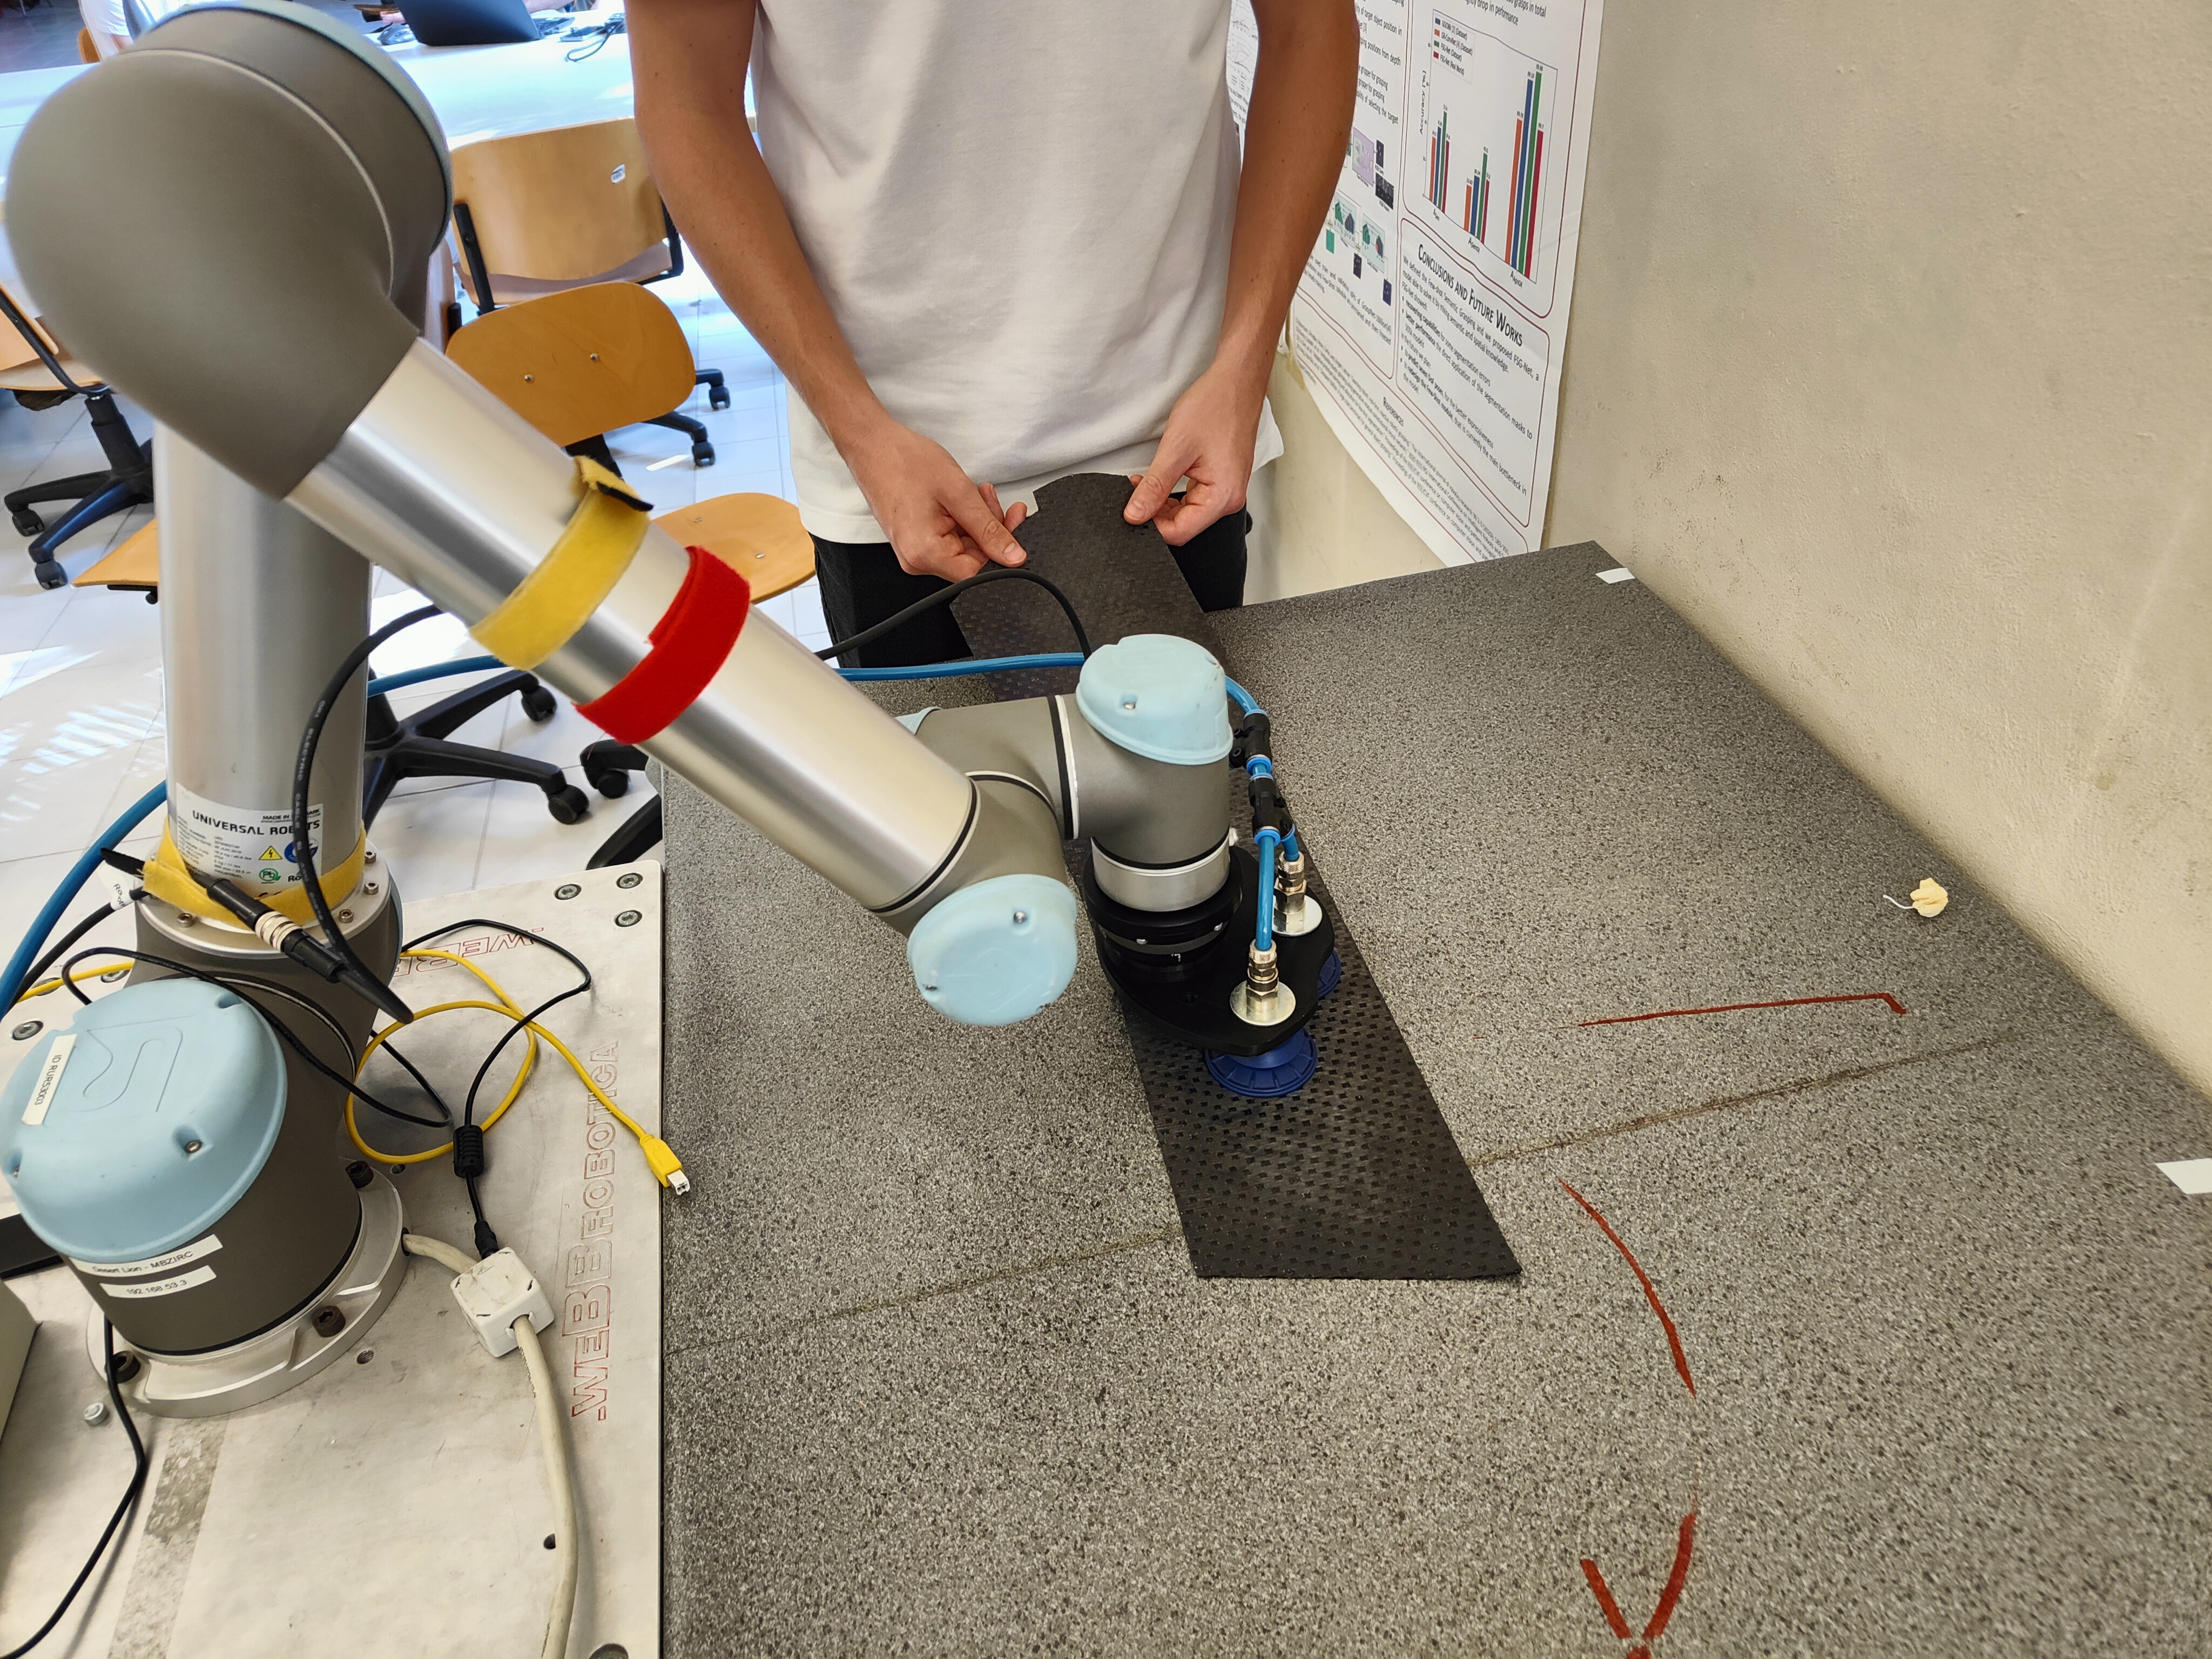
\includegraphics[width=\textwidth]{images/co-op1.jpg}
        \label{fig:co-op1}
    \end{subfigure}
    \qquad
    \begin{subfigure}[b]{0.45\textwidth}
        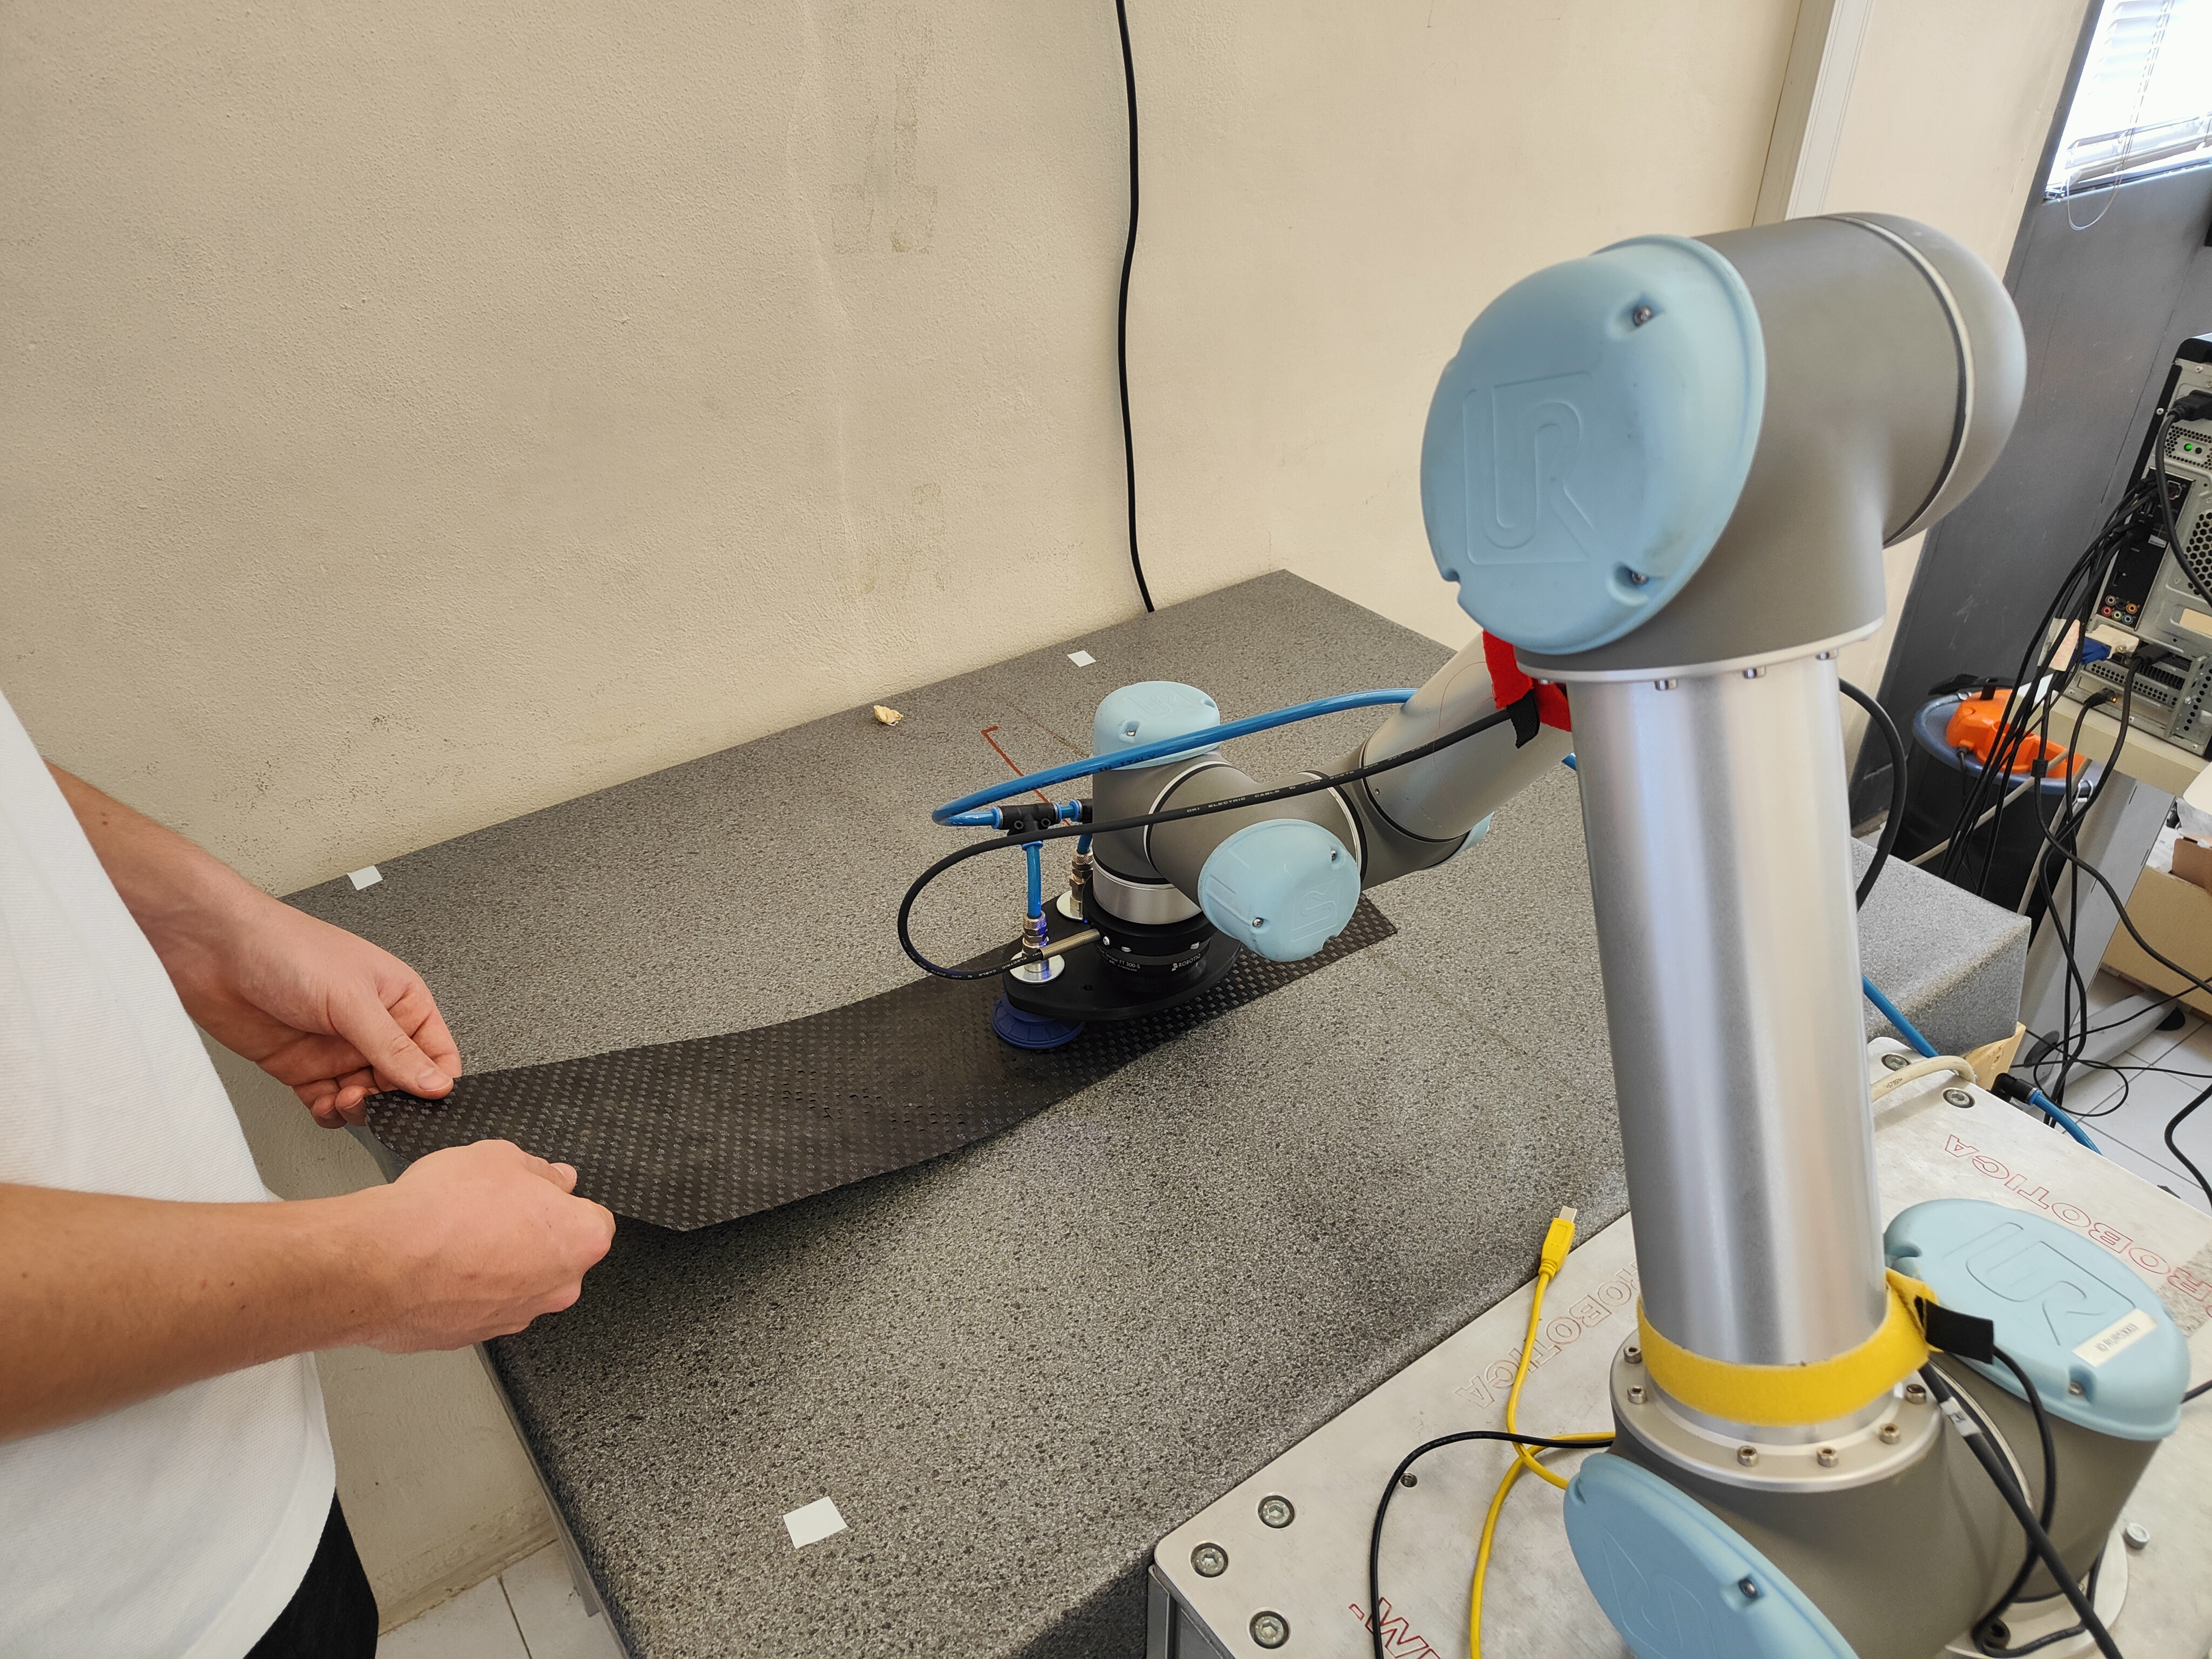
\includegraphics[width=\textwidth]{images/co-op2.jpg}
        \label{fig:co-op2}
    \end{subfigure}
    \caption{Applicazione di trasporto collaborativo, dove il robot segue i movimenti della persona in base alla lettura del sensore di forza}\label{fig:co-op}
\end{figure}
Con l'ausilio dell'\textit{inseguitore di forza}, si potr\'{a} poi trasportare e ruotare la lamina in collaborazione con il robot. 
\footnotetext{\url{https://github.com/andreastocco01/ur5_ft_tasks/blob/main/src/full_velocity_force_follower.cpp}}
